\documentclass[fontsize=12pt]{scrartcl}
\usepackage[ngerman]{babel}
\usepackage[utf8]{inputenc}
%\usepackage[latin1]{inputenc}
\usepackage{amsmath}
\usepackage{amstext}
\usepackage{amssymb}
\usepackage{stmaryrd}
\usepackage{verbatim}
\usepackage{mathrsfs}
\usepackage{extarrows}
\usepackage[arrow, matrix, curve]{xy}
\usepackage[centering,includeheadfoot,margin=2cm]{geometry}
\usepackage{gensymb}
\usepackage{graphicx}
\usepackage{framed}
\usepackage{xcolor}
\usepackage{float}
\usepackage{graphicx} 
\usepackage{sidecap}
\usepackage{blindtext,wrapfig}
\usepackage{epstopdf}
\usepackage{import}
\usepackage{fancyhdr}
\usepackage{fancybox}
\usepackage{graphicx}
\usepackage{caption}
\usepackage{subcaption}
\DeclareGraphicsRule{.tif}{png}{.png}{`convert #1 `basename #1 .tif`.png} 
\pagestyle{fancy}
\fancyhf{}
\fancyhead[R]{Physiklaisches Praktikum 1}
\fancyhead[L]{Linda Werneck, Gentian Rrafshi}
\fancyfoot[R]{Seite \thepage}
\fancyfoot[L]{\today}
\newcommand*{\eqdef}{\stackrel{\scriptscriptstyle\wedge}{=}}
\begin{document}

\begin{minipage}{\textwidth}
\begin{center}\large
\title{M10b Trägheitsmomente aus Drehschwingung \\
		~\\
		~\\
		Assistent: Jonas Binz \\
		Datum Versuchsdurchführung: \\
		29.04.2015}

\author{bearbeitet von\\
		Gruppe 3-031: \\
		Linda Werneck Matrnr. 2901495 \\
		Gentian Rrafshi Matrnr. 2721617 }
\date{\today}

\maketitle

\end{center}
\end{minipage}

\newpage

\tableofcontents

\newpage
\noindent

\section{ Versuchsziel}

Ziel des Versuchs ist die Bestimmung der Winkelrichtwertkonstante und anschließende Berechnung der drei Hauptträgheitsmomente eines isotropen und eines anisotropen Körpers.

\section{ Grundlagen}

Wichtige Grundlage für den Versuch ist die Tatsache, dass über einen starren Körper um jede beliebige Drehachse
\begin{equation*}
J(\omega)=\int r^2 dm
\end{equation*}
als Trägheitsmoment definiert werden kann mit r als Abstand des Massenelements d$m$ von der Drehachse, welche sich mit Winkelgeschwindigkeit $\omega$ bewegt. \\
~\\
Für einen Trägheitsellipsoiden ist das Trägheitsmoment ein Tensor 2. Stufe, d.h. eine $3\times 3$-Matrix. Für die kinetische Energie der Drehbewegung ergibt sich dann also:
\begin{equation*}
E_r=\frac{1}{2} \omega^t \cdot J \cdot \omega = \frac{1}{2} (\omega_x,\omega_y,\omega_z) \left(\begin{array}{ccc}
J_{xx} & J_{xy} & J_{xz} \\ 
J_{yx} & J_{yy} & J_{yz} \\ 
J_{zx} & J_{zy} & J_{zz}
\end{array}\right)  (\omega_x,\omega_y,\omega_z)^t = \frac{1}{2} J(\omega) |\omega|^2
\end{equation*}
Falls $J$ diagonalisierbar ist, ergibt sich durch Hauptachsentransformation und Division mit $J(\omega)$ folgende Gleichung:
\begin{equation*}
\frac{(\omega_x,\omega_y,\omega_z)}{\sqrt{J(\omega)}} \left(\begin{array}{ccc}
J_{xx} & 0 & 0 \\ 
0 & J_{yy} & 0 \\ 
0 & 0 & J_{zz}
\end{array}\right) \frac{ (\omega_x,\omega_y,\omega_z)^t }{\sqrt{J(\omega)}} =1
\end{equation*}
Dies ist die mathematische Beschreibung eines Ellipsoiden.
\newpage

\section{Versuchsaufbau und Durchführung}

Um den Versuch durchführen zu können benötigt man:
\begin{itemize}
\item[1] Kugel mit Bohrungen auf drei zueinander senkrecht stehenden Seiten
\item[2] 5 Stangen, die in die Bohrungen der Kugel eingeschraubt werden können
\item[3] 4 Massen (zwei jeweils gleich große), die man auf den Stangen verschiebbar aufsteckt kann
\item[4] Schneckenfeder
\item[5 ]Federkraftmesser
\item[6] Stoppuhr

\end{itemize}

\subsection{Versuchsaufbau und -Durchführung}
\begin{figure}[H]
        \centering
        \begin{subfigure}[H]{0.4\textwidth}
                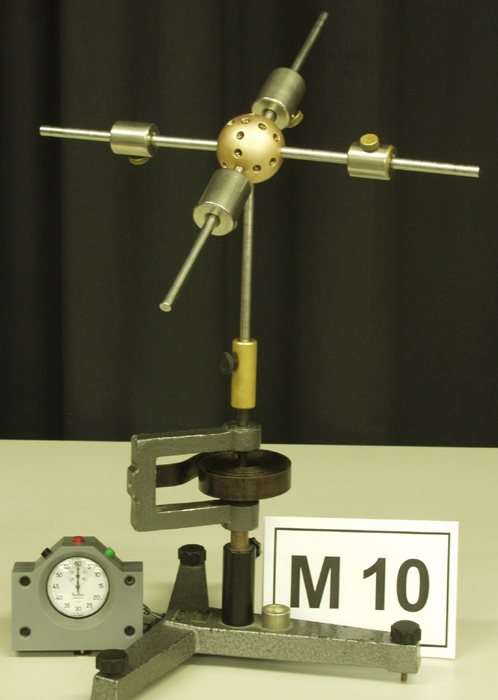
\includegraphics[scale=0.7]{Graphik/Versuchsaufbau}
                \caption{Foto Versuchsaufbau$^{\cite{B}}$}
        \end{subfigure}%
        \begin{subfigure}[H]{0.4\textwidth}
                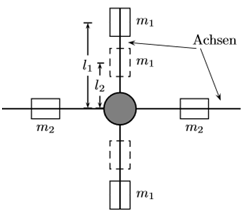
\includegraphics[width=\textwidth]{Graphik/Versuchsaufbau2}
                \caption{Skizze Versuchsaufbau$^{\cite{B}}$}
        \end{subfigure}
\end{figure}
\noindent
\newpage
\subsection{Bestimmung der Winkelrichtgröße D'} 
Vier Stangen werden wie in Abbildung (b) an die Kugel geschraubt. Die fünfte Stange steckt senkrecht zu den anderen in der Kugel und wird mit der Schneckenfeder verbunden (Abbildung (a)).
Die Winkelrichtgröße D' wird mit zwei Methoden bestimmt:

\subsubsection{Statische Methode}
Zwei gleich große Massen werden mit gleichem Abstand zum Kugelmittelpunkt auf zwei gegenüber liegende Stäbe gesteckt. Mit einem Federkraftmesser wird der Körper aus der Ruhelage um eine komplette Drehung senkrecht zur Verbindungsstange gedreht.

\subsubsection{Dynamische Methode}
Die Schwingungsdauer von zwei unterschiedlichen Systemen wird gemessen. Zunächst misst man die Zeit, die das System ohne Gewicht für fünf Perioden braucht. Diese Messung führt man drei Mal durch.  \\
Das zweite System hat den gleichen Aufbau wie das System in 3.2.1. Auch bei diesem System misst die Zeit, die das System für fünf Perioden braucht, drei mal. Aus den Messwerten kann die Winkelrichtgröße berechnet werden

\subsection{Messungen am symmetrischen, anisotropen Körper}
Es muss ein symmetrischer und anisotroper Körper konstruiert werden. Dazu steckt man jeweils zwei gleich große Massen mit gleichem Abstand zur Kugelmitte an die Stäbe gegenüber voneinander. Die kleineren Massen schiebt man auf den Stäben weiter nach innen als die größeren. \\~\\
Die Schwingungsdauer des Körpers um verschiedene Achsen wird nun gemessen. Die Achse wird eingestellt, indem man die fünfte Stange in die unterschiedlichen Bohrungen der Kugel einschraubt. \\
Dabei muss genau notiert werden, um welche Bohrung es sich bei welcher Messung handelt, damit man später die Hauptträgheitsmomente bestimmen kann.
Die Messung um jede Achse wird dreimal wiederholt. Man misst dabei die Zeit, die zehn Periodendauern in Anspruch nehmen.

\subsection{Messungen am symmetrischen, isotropen Körper}
Es wird ein isotroper Körper konstruiert. Dazu variiert man die Abstände der Gewichte zur Kugelmitte so, dass das System um die zwei Achsen, an denen die Massen befestigt sind, die gleichen Periodendauern hat. \\
Die Messung wird analog zum anisotropen Körper an den verschiedenen Achsen mehrmals durchgeführt.

\newpage

\section{ Formeln}
\subsection{Berechnung der Schwingungsdauer pro Periode}
\begin{equation}
\bar{T}= \frac{\sum_{k=1}^n T_k}{n \cdot p}
\end{equation}
Hier ist $T_k$ die jeweilige Schwingungsdauer pro $p$ Perioden für insgesamt $n$ Messungen.
\subsection{Berechnung der Winkelrichtgröße}
\subsubsection{statische Methode} 
\begin{equation}
 D'=\frac{M}{\varphi}= \frac{F \cdot l}{\varphi}
\end{equation}
Wobei $D'$: Winkelrichtgröße, $F$: Kraft, die für eine Umdrehung benötigt wird, l: Abstand zwischen Massemittelpunkt und Kugelmittelpunkt, $\varphi$ : Auslenkung (in diesem Fall 360$^\circ$)
\subsubsection{dynamische Methode}
\begin{equation}
D'=\frac{8 \cdot \pi^2 \cdot m \cdot (l_1^2 – l_2^2)}{T_1^2 – T_2^2}
\end{equation}
Hierbei ist $m_{\text{klein}}$ die Masse des kleinen Masse und  $m_{\text{groß}}$ die Masse des großen Gewichts, $T_1, T_2$: Schwingungsdauer von System ein und zwei, $l_1,l_1$ Abstände der Massen zum Kugelmittelpunkt
\subsection{Berechnung für die Trägheitsmomente J}
\begin{equation}
J(\omega)=\left ( \frac{T(\omega)}{2 \cdot \pi }\right)^2 \cdot D'
\end{equation}
J: Trägheitsmoment

\newpage

\section{ Messwerte}
\begin{figure}[h!]
\vspace{-10pt}
\centering
\caption{Messwerte statische Methode}
\begin{tabular}{|c|c|c|c|c|c|} \hline
Länge l in [cm] & Kraft F in [N]\\ \hline
15&	1,3\\ \hline
\end{tabular}
\end{figure}
\begin{figure}[h!]
\vspace{-10pt}
\centering
\caption{Messwerte dynamische Methode}
\begin{tabular}{|c|c|c|c|c|c|} \hline
 &\multicolumn{5}{|c|}{Schwingungsdauer in [s] über 5 Perioden}\\ \hline
Länge [cm] &1. Messung	&2. Messung	&3. Messung&4. Messung&5. Messung\\ \hline
0&10&	9	&10	&10	&10\\ \hline
15&18&	17,5	&17,4	&17,4	&17,4\\ \hline
\end{tabular}
\end{figure}
\begin{figure}[h!]
\vspace{-10pt}
\centering
\caption{Messwerte für anisotrope Verteilung}
\begin{tabular}{|c|c|c|c|} \hline
&\multicolumn{3}{|c|}{Schwingungsdauer in [s] über 10 Perioden}\\ \hline
Bohrung &1. Messung	&2. Messung	&3. Messung\\ \hline
A		&32,94	&33,02	&32,97	\\ \hline
B		&32,18	&32,06	&32,06	\\ \hline
C		&30,00	&30,09	&29,66	\\ \hline
D		&28,09	&28,85	&28,59	\\ \hline
12	&26,25	&26,47	&26,78	\\ \hline
11		&21,32	&21,18	&21,25	\\ \hline
10	&17,87	&18,00	&17,91	\\ \hline
 c		&22,50	&22,82	&22,66	\\ \hline
 b		&30,22	&30,18	&30,25	\\ \hline
\end{tabular}
\end{figure}
\begin{figure}[h!]
\vspace{-10pt}
\centering
\caption{Messwerte für isotrope Verteilung}
\begin{tabular}{|c|c|c|c|} \hline
 &\multicolumn{3}{|c|}{Schwingungsdauer in [s] über 10 Perioden}\\ \hline
Bohrung &1. Messung	&2. Messung	&3. Messung\\ \hline
A		&33,66&	33,59	&33,44 \\ \hline
B		&31,82&	31,97	&31,85\\ \hline
C		&27,32&	27,18	&27,25\\ \hline
D		&24,32&	24,22	&24,18\\ \hline
12	&24,09&	24,18	&24,06\\ \hline
11		&23,94&	23,82	&23,32\\ \hline
10	&24,44&	24,13	&24,32\\ \hline
 c		&26,85&	27,06	&27,00\\ \hline
 b		&31,94&	31,82	&31,85\\ \hline
\end{tabular}
\end{figure}
\newpage

\section{ Auswertung}
\subsection{Berechnung der Schwingungsdauer pro Periode}
Hier ist $T_k$ die jeweilige Schwingungsdauer pro $p$ Perioden für insgesamt $n$ Messungen.
Zuallererst benötigen wir die Formel (1) um die Mittlere Schwingungsdauer zu berechnen:
\begin{equation*}
\bar{T}= \frac{\sum\limits_{k=1}^n T_k}{n \cdot p}
\end{equation*}
Als Beispiel wird hier $\bar{T}$ bei $0\,\text{cm}$ für die dynamische Methode zur Berechnung von $D'$ berechnet.
\begin{equation*}
\bar{T}= \frac{\sum\limits_{k=1}^n T_k}{n \cdot p}= \frac{10\,\text{s} + 9\,\text{s} + 10\,\text{s} + 10\,\text{s} + 10\,\text{s}}{5 \cdot 5}=1,96\,\text{s}
\end{equation*}
\begin{figure}[h!]
\vspace{-10pt}
\centering
\caption{Auswertung dynamische Methode}
\begin{tabular}{|c|c|} \hline
\rule{0pt}{12,5pt}Länge [cm] &mittlere Schwingungsdauer $\bar{T}$ in [s]	\\ \hline
0		&1,96	\\ \hline
15	&3,51	\\ \hline
\end{tabular}
\end{figure}
\begin{figure}[h!]
\vspace{-10pt}
\centering
\caption{Auswertung  für anisotrope und isotrope Verteilung}
\begin{tabular}{|c|c|c|c|} \hline
\rule{0pt}{12,5pt}&\multicolumn{2}{c|}{mittlere Schwingungsdauer $\bar{T}$ in [s]}\\ \hline
Bohrung & anisotrope Verteilung & isotrope Verteilung\\ \hline
A		&	3,30&3,36	\\ \hline
B		&3,21&3,19	\\ \hline
C		&2,99&2,73	\\ \hline
D		&2,85&2,42	\\ \hline
12	&2,65&2,41	\\ \hline
11		&2,13&2,37	\\ \hline
10	&1,79&2,43	\\ \hline
 c		&2,27&2,70	\\ \hline
 b		&3,02&3,19	\\ \hline
\end{tabular}
\end{figure}

\subsection{ Auswertung der Winkelrichtgröße}
\subsubsection{statische Methode} 
Für die statische Methode zur Berechnung der Winkelrichtgröße nutzen wir Formel (2) aus. Daraus ergibt sich für $\varphi=360^{\circ} \eqdef 2\pi$.
\begin{equation*}
 D'=\frac{M}{\varphi}= \frac{F \cdot l}{\varphi} = \frac{1,3\,\text{N} \cdot 0,15\,\text{m} }{2\pi} = 0,0310\,\text{Nm}
\end{equation*}

\subsubsection{dynamische Methode}
Bei der dynamischen Methode können wir mit Hilfe von Formel (3) die Winkelrichtgröße ausrechnen.
\begin{equation*}
D'=\frac{8 \cdot \pi^2 \cdot m_{\text{klein}} \cdot (l_1^2 – l_2^2)}{T_1^2 – T_2^2} = \frac{8 \cdot \pi^2 \cdot  0,109\,\text{kg} \cdot (0,15\,\text{m})^2}{(3,51\,\text{s})^2 – (1,96\,\text{s})^2} = 0,023\,\text{Nm}
\end{equation*}

\subsection{ Auswertung für die Trägheitsmomente J}
\begin{figure}[h!]
\begin{minipage}{\textwidth}
\begin{wrapfigure}{l}{0.35\textwidth}
	\vspace{-20pt}
                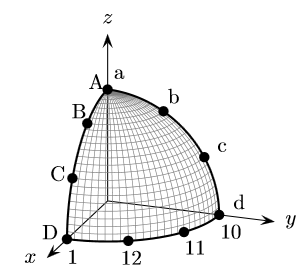
\includegraphics[scale=0.7]{Graphik/Kugel-Oktant}             
			\caption{Kugel-Oktant$^{\cite{C}}$}
	\end{wrapfigure}
Ein weiteres Ziel des Versuchs ist es, die Hauptträgheitsmomente $J_x,J_y,J_z$ auszurechnen. Da wir uns während des Versuchs nach dem Kugel-Oktanten in Abbildung. 
(8) gerichtet haben, sieht man nun sehr leicht, dass unsere Hauptträgheitsmomente an den Bohrungen A,D,10 sind. Nun können wir mit Hilfe von Formel (4) 
\begin{equation*}
J(\omega)=\left ( \frac{T(\omega)}{2 \cdot \pi }\right)^2 \cdot D'
\end{equation*}
die Hauptträgheitsmomente berechnen.
\end{minipage}
\end{figure}
\subsubsection{Auswertung des Trägheitsmomentes J für anisotrope Verteilung}
Für die Berechnung der jeweiligen Hauptträgheitsmomente benötigen wir als die Schwingungsdauer an den Bohrungen D für $J_x$, 10 für $J_y$ und A für $J_z$ und erhalten somit mit $D'= 0,01143\,\text{Nm}$.
\begin{align*}
J_x(\omega) &=\left ( \frac{T_x(\omega)}{2 \cdot \pi }\right)^2 \cdot D' = \left ( \frac{2,85\,\text{s}}{2 \cdot \pi }\right)^2 \cdot  0,023\,\text{Nm}
=0,46\,\text{kg$\cdot$m$^2$} \\
J_y(\omega) &=\left ( \frac{T_y(\omega)}{2 \cdot \pi }\right)^2 \cdot D' = \left ( \frac{1,79\,\text{s}}{2 \cdot \pi }\right)^2 \cdot  0,023\,\text{Nm}
=0,18\,\text{kg$\cdot$m$^2$} \\
J_z(\omega) &=\left ( \frac{T_z(\omega)}{2 \cdot \pi }\right)^2 \cdot D' = \left ( \frac{3,30\,\text{s}}{2 \cdot \pi }\right)^2 \cdot  0,023\,\text{Nm}
=0,62\,\text{kg$\cdot$m$^2$} \\
\end{align*}
\subsubsection{Auswertung des Trägheitsmomentes J für isotrope Verteilung}
Analog zu 6.2.1 Berechnen wir auch für den isotropen Körper die Hauptträgheitsmomente
\begin{align*}
J_x(\omega) &=\left ( \frac{T_x(\omega)}{2 \cdot \pi }\right)^2 \cdot D' = \left ( \frac{2,42\,\text{s}}{2 \cdot \pi }\right)^2 \cdot  0,023\,\text{Nm}
=0,34\,\text{kg$\cdot$m$^2$} \\
J_y(\omega) &=\left ( \frac{T_y(\omega)}{2 \cdot \pi }\right)^2 \cdot D' = \left ( \frac{2,43\,\text{s}}{2 \cdot \pi }\right)^2 \cdot  0,023\,\text{Nm}
=0,34\,\text{kg$\cdot$m$^2$} \\
J_z(\omega) &=\left ( \frac{T_z(\omega)}{2 \cdot \pi }\right)^2 \cdot D' = \left ( \frac{3,36\,\text{s}}{2 \cdot \pi }\right)^2 \cdot  0,023\,\text{Nm}
=0,64\,\text{kg$\cdot$m$^2$} \\
\end{align*}
\noindent
Auch war es unsere Aufgabe, einen Plot zu erstellen in dem in Abhängigkeit von den Bohrlöchern eine zu $\frac{1}{\sqrt J}$ proportionale Größe aufgetragen wird. Aus Formel (4) ergibt sich dafür $\frac{1}{T}$, für uns ergibt sich dadurch folgender Plot:

\begin{figure}[h!]
\centering
  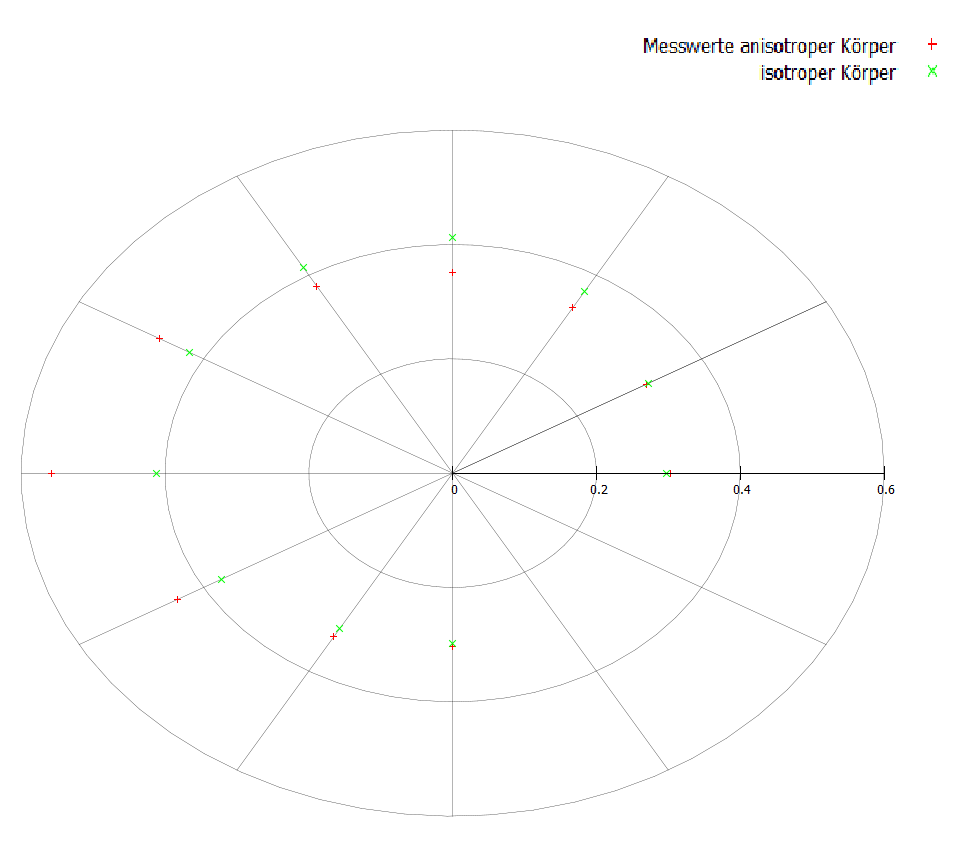
\includegraphics[scale=0.5]{Graphik/plot}
                \caption{$\frac{1}{T}$ an jedem Bohrloch }
\end{figure}
\newpage
\noindent
\section{Fehlerrechnung}

\subsection{Fehlerquellen}

In diesem Versuch wird viel gemessen und man hat dementsprechend viele Messungenauigkeiten.
Das Messen mit dem Lineal hat einen Fehler $\Delta l$ von $1$\,mm und die Messungenauigkeit beim Zeitmessen mit der Stoppuhr hat die übliche 
menschliche Reaktionszeit von $\Delta t$ von $1$\,s. Beim wiegen der Gewichte kann eine Fehler von $1$\,g angenommen werden. 
Ein weiterer Fehler bei der statischen Methode ist beim drehen um 360$^{\circ}$, was nun eher ein drehen im Kreis war und deswegen hier auch ein Fehler, 
der auf 10$^{\circ}$ geschätzt wird. Zudem kann für den Kraftmesser ein Fehler von 0,01\,N angenommen werden.

\subsection{Fehlerrechnung}

\subsubsection{Fehler bei der Schwingungsdauer pro Periode}
Da wir bei der Zeitmessung die Reaktionszeit des Menschen mit einberechnen müssen, erhalten wir also insgesamt 
\begin{align*}
\Delta \bar{T}&=\left \vert\frac{\partial}{\partial T_k} \frac{\sum\limits_{k=1}^n T_k}{n \cdot p} \cdot \Delta t \right \vert\\
&=\left \vert  \frac{\sum\limits_{k=1}^n }{n \cdot p} \cdot \Delta t \right \vert =\left \vert  \frac{1+1+1+1+1}{n \cdot p} \cdot \Delta t \right \vert\\
&=\left \vert \frac{5\cdot 1\,\text{s}}{5 \cdot 5}\right \vert=\frac{1}{5}\,\text{s}=0,2\,\text{s}
\end{align*}
bzw. $0,1\,\text{s}$ wenn über 10 Perioden gemessen wird.
Hierbei ist zu beachten, dass der Fehler bei der Mittelwertbildung gleich bleibt und sich nur bei der Periodendauer reduziert.
\subsubsection{ Fehler bei der Winkelrichtgröße}
Bei der statische Methode zur Berechnung der Winkelrichtgröße ergibt sich für $\varphi=360^{\circ} \eqdef 2\pi$ folgender Fehler:
\begin{align*}
\Delta D'&=\left \vert\frac{\partial}{\partial F} \frac{F \cdot l}{\varphi} \cdot \Delta F \right \vert + \left \vert\frac{\partial}{\partial l} \frac{F \cdot l}{\varphi}  \cdot \Delta l  \right \vert \\
&=\left \vert \frac{\Delta F \cdot l}{\varphi}  \right \vert + \left \vert \frac{F \cdot  \Delta l}{\varphi} \right \vert \\
&=\left \vert \frac{0,01\,\text{N} \cdot 0,15\,\text{m}}{2\pi}  \right \vert + \left \vert \frac{0,65\,\text{N} \cdot  0,001 \text{m}}{2\pi} \right \vert \\
&=\left \vert 0,00235619449  \right \vert +\left \vert 0,00102101761 \right \vert = 0,003\,\text{Nm}
\end{align*}
\newpage
\noindent
Bei der dynamischen Methode erhalten wir einen Fehler wie folgt, wobei wegen $l_1=0\,\text{cm}$ können wir annehmen, dass dort kein Fehler existiert:
\begin{align*}
\Delta D'&=\left \vert \frac{\partial}{\partial m_{\text{klein}}} \frac{4 \cdot \pi^2 \cdot m_{\text{klein}} \cdot (l_1^2 – l_2^2)}{T_1^2 – T_2^2} \cdot 
\Delta m_{\text{klein}} \right \vert 
+\left \vert\frac{\partial}{\partial l_2} \frac{4 \cdot \pi^2 \cdot m_{\text{klein}} \cdot (l_1^2 – l_2^2)}{T_1^2 – T_2^2} 
\cdot \Delta l_2 \right \vert \\
&+ \left \vert\frac{\partial}{\partial T_1} \frac{4 \cdot \pi^2 \cdot m_{\text{klein}} \cdot (l_1^2 – l_2^2)}{T_1^2 – T_2^2} \cdot 
\Delta T_1 \right \vert
+ \left \vert\frac{\partial}{\partial T_2} \frac{4 \cdot \pi^2 \cdot m_{\text{klein}} \cdot (l_1^2 – l_2^2)}{T_1^2 – T_2^2} \cdot 
\Delta T_2 \right \vert\\
%
&=\left \vert  \frac{4 \cdot \pi^2 \cdot \Delta m_{\text{klein}} \cdot (l_1^2 – l_2^2)}{T_1^2 – T_2^2} \right \vert 
+\left \vert \frac{4 \cdot \pi^2 \cdot m_{\text{klein}} \cdot (l_1^2 – \Delta l_2^2)}{T_1^2 – T_2^2}  \right \vert \\
&+ \left \vert- \frac{4 \cdot \pi^2 \cdot m_{\text{klein}} \cdot (l_1^2 – l_2^2)\cdot T_1}{(T_1^2 – T_2^2)^2} \cdot 
\Delta T_1 \right \vert
+\left \vert \frac{4 \cdot \pi^2 \cdot m_{\text{klein}} \cdot (l_1^2 – l_2^2)\cdot T_2}{(T_1^2 – T_2^2)^2} \cdot 
\Delta T_2 \right \vert \\
%
&=\left \vert  \frac{4 \cdot \pi^2 \cdot 0,001\,\text{kg} \cdot (0,15\,\text{m})^2}{(3,51\,\text{s})^2 – (1,96\,\text{s})^2} \right \vert 
+\left \vert \frac{4 \cdot \pi^2 \cdot 0,109\,\text{kg} \cdot (0,001\,\text{m}\cdot 2 \cdot 0,15\,\text{m})}{(3,51\,\text{s})^2 – (1,96\,\text{s})^2}  \right \vert \\
&+ \left \vert- \frac{4 \cdot \pi^2 \cdot 0,109\,\text{kg} \cdot(0,15\,\text{m})^2\cdot 3,51\,\text{s}\cdot 2}{((3,51\,\text{s})^2 – (1,96\,\text{s})^2)^2} \cdot 
0,2\,\text{s} \right \vert\\
&+\left \vert \frac{4 \cdot \pi^2 \cdot 0,109\,\text{kg} \cdot (0,15\,\text{m})^2\cdot 1,96\,\text{s}\cdot 2}{((3,51\,\text{s})^2 – (1,96\,\text{s})^2)^2} \cdot 
0,2\,\text{s} \right \vert \\
%
&=0,00010\,\text{Nm}+ 0,00015\,\text{Nm} + 0,00189\,\text{Nm} +0,00106\,\text{Nm} =   0,003\,\text{Nm}
\end{align*}
\subsubsection{ Fehler für die Trägheitsmomente J}
Zu guter Letzt berechnen wir noch den Fehler bei den Hauptträgheitsmomenten wie folgt beispielhaft für $J_x$:
\begin{align*}
\Delta J_x(\omega) &=\left \vert  \frac{\partial}{\partial T_x(\omega) } \left(\frac{T_x(\omega)}{2 \cdot \pi }\right)^2 \cdot D' \right \vert
+ \left \vert  \frac{\partial}{\partial D' } \left(\frac{T_x(\omega)}{2 \cdot \pi }\right)^2 \cdot D' \right \vert \\
&=\left \vert  \left(\frac{2 \cdot T_x(\omega) \cdot \Delta T_x(\omega)}{(2 \cdot \pi)^2 }\right) \cdot D' \right \vert
+ \left \vert  \left(\frac{T_x(\omega)}{2 \cdot \pi }\right)^2 \cdot \Delta D' \right \vert \\
&=\left \vert  \left(\frac{2 \cdot 2,85\,\text{s} \cdot 0,1\,\text{s}}{(2 \cdot \pi)^2 }\right) \cdot 0,01143\,\text{Nm} \right \vert
+ \left \vert  \left(\frac{2,85\,\text{s}}{2 \cdot \pi }\right)^2 \cdot 0,003\,\text{Nm} \right \vert \\
&=0,00017\,\text{kg$\cdot$m$^2$} +0,06\,\text{kg$\cdot$m$^2$} = 0,06\,\text{kg$\cdot$m$^2$} \\
\end{align*}
Für die anderen Trägheitsmomente ergibt sich:
\begin{align*}
\Delta J_y(\omega)  = 0,02\,\text{kg$\cdot$m$^2$} \\
\Delta J_z(\omega) = 0,08\,\text{kg$\cdot$m$^2$}
\end{align*}
\newpage
\noindent
und analog noch für die isotropen Verteilung:
\begin{align*}
\Delta J_x(\omega) = 0,04\,\text{kg$\cdot$m$^2$} \\
\Delta J_y(\omega) = 0,04\,\text{kg$\cdot$m$^2$} \\
\Delta J_z(\omega) = 0,08\,\text{kg$\cdot$m$^2$}
\end{align*}
Bei den Hauptträgheitsmomenten haben wir immer einen Fehler von $\approx 25\%$. Schon bei den Schwingungsdauern haben wir teilweise Fehler bis zu $\approx 10\%$. Die Fehler könnten minimiert werden, in dem man z.B. über mehr Perioden geht. So würde der Fehler bei der Schwingungsdauer kleiner werden. Auch würden eine genauere Waage, genaueres Lineal helfen, um Messfehler generell klein zu halten.

\section{Zusammenfassung}

Ziel des Versuchs war es die Winkelrichtgröße und die Hauptträgheitsmomenten zu bestimmen.
Dafür wurde zuerst die Schwingungsdauer bestimmt. In den nachfolgenden Tabellen sind alle Schwingungsdauern mit Fehler aufgeführt.
\begin{figure}[h!]
\vspace{-10pt}
\centering
\caption{Auswertung dynamische Methode}
\begin{tabular}{|c|c|} \hline
\rule{0pt}{12,5pt}Länge [cm] &mittlere Schwingungsdauer $\bar{T}+ \Delta t$ in [s]	\\ \hline
0		&1,96$\pm$ 0,2\\ \hline
15	&3,51$\pm$ 0,2	\\ \hline
\end{tabular}
\end{figure}
\begin{figure}[h!]
\vspace{-10pt}
\centering
\caption{Auswertung  für anisotrope und isotrope Verteilung}
\begin{tabular}{|c|c|c|c|} \hline
\rule{0pt}{12,5pt}&\multicolumn{2}{c|}{mittlere Schwingungsdauer $\bar{T}+\Delta t$ in [s]}\\ \hline
Bohrung & anisotrope Verteilung & isotrope Verteilung\\ \hline
A		&	3,30$\pm$ 0,1&3,36$\pm$ 0,1	\\ \hline
B		&3,21$\pm$ 0,1&3,19$\pm$ 0,1	\\ \hline
C		&2,99$\pm$ 0,1&2,73$\pm$ 0,1	\\ \hline
D		&2,85$\pm$ 0,1&2,42$\pm$ 0,1	\\ \hline
12	&2,65$\pm$ 0,1&2,41$\pm$ 0,1	\\ \hline
11		&2,13$\pm$ 0,1&2,37$\pm$ 0,1	\\ \hline
10	&1,79$\pm$ 0,1&2,43$\pm$ 0,1	\\ \hline
 c		&2,27$\pm$ 0,1&2,70$\pm$ 0,1	\\ \hline
 b		&3,02$\pm$ 0,1&3,19$\pm$ 0,1	\\ \hline
\end{tabular}
\end{figure}
\noindent
Für die Bestimmung der Winkelrichtgröße gab es zwei Methoden, die statische und dynamische Methode.
Wir bekamen bei unserem Versuch dafür folgende Winkelrichtgrößen mit Fehler:
\begin{align*}
D'_{\text{statisch}}+\Delta D'_{\text{statisch}}&= 0,01553\,\text{Nm}\pm0,003\,\text{Nm} \\
D'_{\text{dynamisch}}+\Delta D'_{\text{dynamisch}}&= 0,01143\,\text{Nm}\,\text{Nm}\pm0,003\,\text{Nm}
\end{align*}
Wie in der Auswertung angemerkt, sind die Werte ziemlich nah beianander und für diesen Versuch hätten wir genauso für die Auswertung der Hauptträgheitsmomente $D'_{\text{statisch}}$ nehmen können.
\newpage
\noindent
Zu guter Letzt wurden die Hauptträgheitsmomente jeweils für einen anisotropen und isotropen Körper ausgerechnet: 
Diese waren im anisotropen Fall:
\begin{align*}
J_x(\omega)+\Delta J_x(\omega) &=0,23\,\text{kg$\cdot$m$^2$}\pm 0,06\,\text{kg$\cdot$m$^2$} \\
J_y(\omega)+\Delta J_y(\omega) &=0,09\,\text{kg$\cdot$m$^2$}\pm 0,02\,\text{kg$\cdot$m$^2$} \\
J_z(\omega)+\Delta J_z(\omega) &=0,31\,\text{kg$\cdot$m$^2$}\pm  0,08\,\text{kg$\cdot$m$^2$}\\
\end{align*}
und im isotropen Fall:
\begin{align*}
J_x(\omega)+\Delta J_x(\omega) &=0,17\,\text{kg$\cdot$m$^2$}\pm  0,04\,\text{kg$\cdot$m$^2$}\\
J_y(\omega)+\Delta J_y(\omega) &=0,17\,\text{kg$\cdot$m$^2$}\pm  0,04\,\text{kg$\cdot$m$^2$}\\
J_z(\omega)+\Delta J_z(\omega) &=0,32\,\text{kg$\cdot$m$^2$}\pm 0,08\,\text{kg$\cdot$m$^2$} \\
\end{align*}
Bei den Hauptträgheitsmomenten haben wir immer einen Fehler von $\approx 25\%$. Angesichts der vielen Messungenauigkeiten war ein solch hoher prozentualer Fehler zu erwarten,
schon bei den Schwingungsdauern haben wir teilweise Fehler bis zu $\approx 10\%$. 
Die Fehler könnten minimiert werden, in dem man z.B. über mehr Perioden geht. So würde der Fehler bei der Schwingungsdauer kleiner werden. Auch würden eine genauere Waage, genauere Stoppuhr, genaueres Lineal helfen, um Messfehler generell klein zu halten.
\newpage
\section{Literaturverzeichnis}

\begin{thebibliography}{xxxxxxxx}
\bibitem[1]{1}		\textit{\glqq M10 Trägheitsmomente aus Drehschwingung\grqq , in 
								http:www3.physik.uni-stuttgart.de/studium/praktika/ap/},\textit{ unter 
								http://www3.physik.uni-stuttgart.de/studium/praktika/ap/pdf\_dateien/M10.pdf abgerufen am 17.05.2015}
\bibitem[A]{A}  	Graphik aus \textit{\glqq M10 Trägheitsmomente aus Drehschwingung\grqq , in 	http://www3.physik.uni-stuttgart.de/studium/
   								praktika/ap/}, \textit{ unter 	http://www3.physik.uni-stuttgart.de/studium/praktika/ap/bilder/M10.jpg ; abgerufen am 
   								17.05.2015} 

\end{thebibliography}

\section{Anhang}

%\begin{figure}[h]
%\vspace{-20pt}
%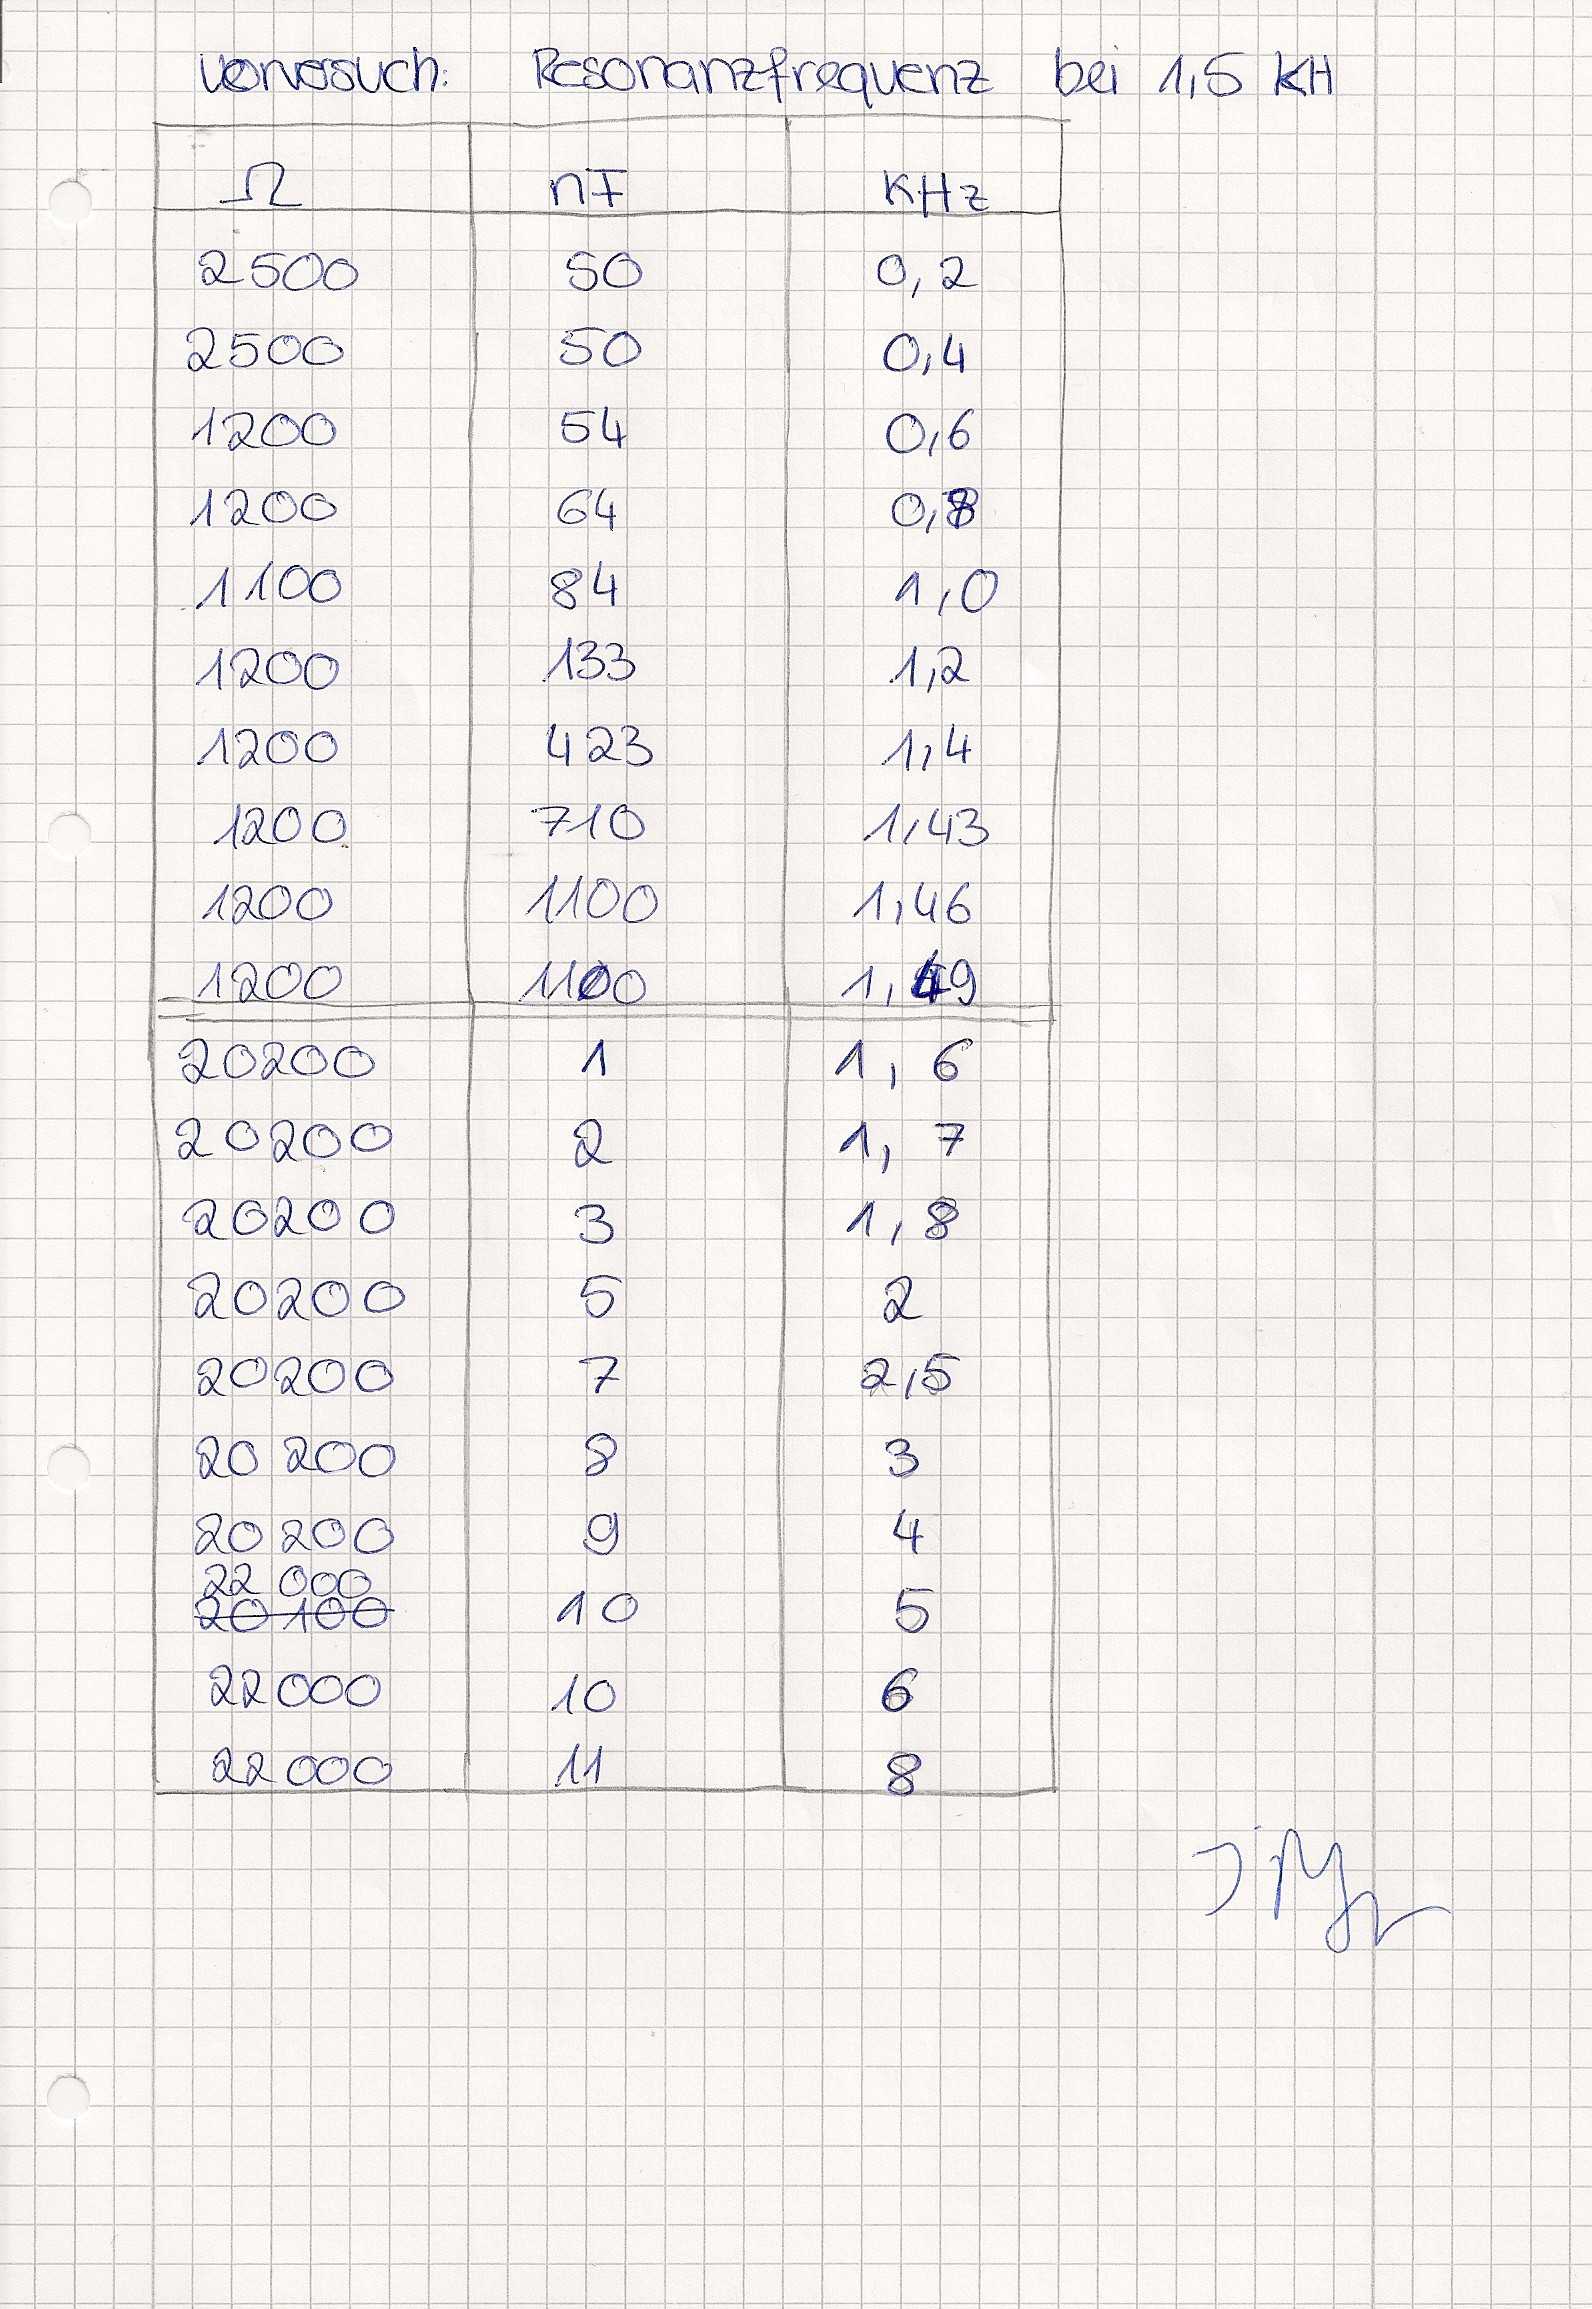
\includegraphics[scale=0.3]{Graphik/Linda}
%\end{figure}

\end{document}